\documentclass[10pt]{article}
\usepackage{mathpaper}

\begin{document}
\showsecret
\anspapertitle{2024年武汉市初中毕业生学业考试(模拟一)}
\informationline \par

\noindent  \ \textbf{\selectingintroduction}
\begin{table}[!htb]
    \centering
    \begin{tabularx}{\textwidth}{|*{11}{>{\centering\arraybackslash}X|}} \hline
        题号 & 1 & 2 & 3 & 4 & 5 & 6 & 7 & 8 & 9 & 10 \\ \hline
        选项 & \quad & \quad & \quad & \quad & \quad & \quad & \quad & \quad & \quad & \quad \\ \hline
    \end{tabularx}
\end{table} \par

\noindent  \ \textbf{\complitingintroduction}
\begin{table}[!htb]
    \centering
    \renewcommand\arraystretch{1.5}
    \begin{tabularx}{\textwidth}{*{3}{>{\centering\arraybackslash}X}}
        11.\complitingline\complitingline\complitingline & 12.\complitingline\complitingline\complitingline & 13.\complitingline\complitingline\complitingline \\
        14.\complitingline\complitingline\complitingline & 15.\complitingline\complitingline\complitingline & 16.\complitingline\complitingline\complitingline  \\
    \end{tabularx}
\end{table}

\setcounter{taskcounter}{16}
\begin{questions}{\answeringintroduction}
    \question %17
    \begin{subquestions}
        \rmsubquestion \complitingline\complitingline
        \rmsubquestion \complitingline\complitingline
        \rmsubquestion \qquad
        \addemptyline
        \begin{figure}[!htb]
            \centering
            \begin{tikzpicture}[>=Stealth,scale=1.2]
                \draw[->] (-4.3,0) -- (4.3,0);
                \foreach \i in {-4,-3,...,4}
                {
                    \draw (\i,0.1) -- (\i,0) node[below] {$\i$};
                }
            \end{tikzpicture}
        \end{figure}
        \rmsubquestion \complitingline\complitingline
    \end{subquestions}
    \question %18
    \begin{subquestions}
        \subquestion \addemptyline\addemptyline
        \subquestion \qquad
        \begin{figure}[!htb]
            \raggedleft
            \subfigure{
                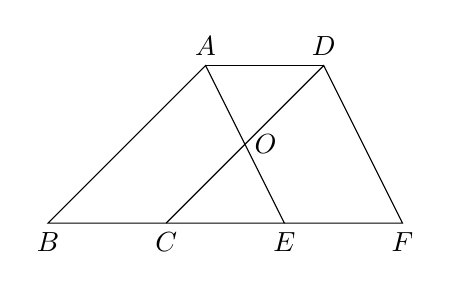
\begin{tikzpicture}[scale=0.5]
                    \coordinate[label=below:{$B$}] (B) at (0,0);
                    \coordinate[label=below:{$C$}] (C) at (3,0);
                    \coordinate[label=below:{$E$}] (E) at (6,0);
                    \coordinate[label=below:{$F$}] (F) at (9,0);
                    \coordinate[label=above:{$A$}] (A) at (4,4);
                    \coordinate[label=above:{$D$}] (D) at (7,4);
                    \coordinate[label=right:{$O$}] (O) at (5,2);
                    \draw (A) -- (B) -- (E) -- cycle;
                    \draw (C) -- (D) -- (F) -- (E);
                    \draw (A) -- (D);
                \end{tikzpicture}
            }
        \end{figure}\addemptyline\addemptyline
    \end{subquestions}
    \question %19
    \begin{subquestions}
        \subquestion \complitingline\complitingline
        \subquestion \complitingline\complitingline;\complitingline\complitingline
        \subquestion \qquad
        \begin{figure}[!htb]
            \centering
            \subfigure{
            \begin{tikzpicture}[>=Stealth,scale=0.125]
                \draw[->] (0,0) -- (45,0) node[below] {观点};
                \draw[->] (0,0) -- (0,30) node[right] {人数/人};
                \foreach \i in {5,10,...,25}
                {
                    \draw[densely dashed] (40,\i) -- (0,\i) node[left] {$\i$};
                }
                \draw (5,0) -- (5,1);
                \draw (10,0) -- (10,1);
                \node[below] at (7.5,0) {A};
                \node[below] at (17.5,0) {B};
                \node[below] at (27.5,0) {C};
                \node[below] at (37.5,0) {D};
                \node[left] at (0,0) {$0$};
                \filldraw[color=white] (15,0) rectangle (20,12);
                \draw (15,0) rectangle (20,12);
                \filldraw[color=white] (25,0) rectangle (30,8);
                \draw (25,0) rectangle (30,8);
                \filldraw[color=white] (35,0) rectangle (40,20);
                \draw (35,0) rectangle (40,20);
                \node[above] at (17.5,12) {$12$};
                \node[above] at (27.5,8) {$8$};
                \node[above] at (37.5,20) {$20$};
            \end{tikzpicture}}
        \end{figure}\newpage
        \subquestion \addspace\addspace
    \end{subquestions}
    \question %20
    \begin{subquestions}
        \subquestion \qquad
        \begin{figure}[!htb]
            \raggedleft
            \subfigure{
            \begin{tikzpicture}[>=Stealth,scale=0.6]
                \coordinate[label=below:{$B$}] (B) at (0,0);
                \coordinate[label=below:{$M$}] (M) at (-1.5,0);
                \coordinate[label=below:{$N$}] (N) at (6.5,0);
                \coordinate[label=below:{$C$}] (C) at (1,0);
                \coordinate[label=below:{$E$}] (E) at (4,0);
                \coordinate[label=left:{$A$}] (A) at (0,2);
                \coordinate[label=above right:{$D$}] (D) at (4,4);
                \draw (M) -- (N);
                \draw (B) -- (A) -- (C) -- (D) -- (E);
                \draw (A) -- (D);
                \draw (2.5,2) circle (2.5);
            \end{tikzpicture}}
        \end{figure}
        \subquestion \addspace\addspace
    \end{subquestions}
    \question \qquad
    \begin{figure}[!htb]
        \raggedleft
        \subfigure[(1)]{
        \begin{tikzpicture}[>=Stealth,scale=0.6]
            \draw[step=1,densely dashed] (0,0) grid (9,6);
            \coordinate[label=above:{$A$}] (A) at (6,6);
            \coordinate[label=right:{$B$}] (B) at (9,2);
            \coordinate[label=below:{$C$}] (C) at (6,0);
            \coordinate[label=right:{$P$}] (P) at (7.23,4.36);
            \draw (A) -- (B) -- (C) -- cycle;
            \filldraw (P) circle (0.05);
        \end{tikzpicture}}\qquad
        \subfigure[(2)]{
        \begin{tikzpicture}[>=Stealth,scale=0.6]
            \draw[step=1,densely dashed] (0,0) grid (9,6);
            \coordinate[label=above:{$A$}] (A) at (6,6);
            \coordinate[label=right:{$B$}] (B) at (9,2);
            \coordinate[label=below:{$C$}] (C) at (6,0);
            \coordinate[label=right:{$P$}] (P) at (7.23,4.36);
            \draw (A) -- (B) -- (C) -- cycle;
            \filldraw (P) circle (0.05);
        \end{tikzpicture}}\qquad
    \end{figure}
    \question \begin{enumerate}[topsep=0.5pt,parsep=0.5pt,itemsep=0.5pt,leftmargin=57.5pt,rightmargin=6pt]
        \item[\textbf{探究发现} \quad] \complitingline\complitingline;\complitingline\complitingline \newpage
        \item[\textbf{问题解决} \quad]
    \begin{subquestions}
        \subquestion \addspace
        \subquestion \qquad
        \begin{figure}[!htb]
            \raggedleft
            \subfigure{
            \begin{tikzpicture}[>=Stealth,scale=0.5]
                \draw[->] (-0.5,0) -- (10,0) node[below] {$x$};
                \draw[->] (0,-0.5) -- (0,5) node[right] {$y$};
                \coordinate[label=below left:{$A$}] (A) at (0,0);
                \draw (0,3) parabola bend (3,4) (8.5,0);
                \draw[line width =1pt] (8,0) -- (9,0);
                \coordinate[label=below:{$M$}] (M) at (8,0);
                \coordinate[label=below:{$N$}] (N) at (9,0);
            \end{tikzpicture}}
        \end{figure}\addemptyline\addemptyline\addemptyline
    \end{subquestions}
    \end{enumerate}
    \question \begin{enumerate}[topsep=0.5pt,parsep=0.5pt,itemsep=0.5pt,leftmargin=57.5pt,rightmargin=6pt]
        \item[\textbf{问题探究} \quad]
            \begin{subquestions}
                \subquestion $\frac{AB}{AE}+\frac{AC}{AF}=$\complitingline\complitingline
                \subquestion \qquad
                \begin{figure}[!htb]
                    \raggedleft
                    \subfigure{
                    \begin{tikzpicture}[>=Stealth,scale=0.5]
                        \coordinate[label=left:{$B$}] (B) at (0,0);
                        \coordinate[label=above:{$A$}] (A) at (5,4);
                        \coordinate[label=right:{$C$}] (C) at (6,0);
                        \coordinate[label=below:{$D$}] (D) at (3,0);
                        \coordinate[label=above left:{$E$}] (E) at (1.25188,1.00151);
                        \coordinate[label=below right:{$F$}] (F) at (6.50151,-2.00603);
                        \draw (A) -- (B) -- (C) -- cycle;
                        \draw (A) -- (D);
                        \draw (E) -- (F) -- (C);
                    \end{tikzpicture}}
                \end{figure}\addemptyline\addemptyline\addemptyline
            \end{subquestions}
        \item[\textbf{问题拓展} \quad] \qquad
                \begin{figure}[!htb]
                    \raggedleft
                    \subfigure{
                    \begin{tikzpicture}[>=Stealth,scale=0.6]
                        \coordinate[label=left:{$B$}] (B) at (0,0);
                        \coordinate[label=above:{$A$}] (A) at (6,4);
                        \coordinate[label=right:{$C$}] (C) at (6,0);
                        \coordinate[label=below:{$D$}] (D) at (3,0);
                        \coordinate[label=right:{$F$}] (F) at (6,2.11675);
                        \coordinate[label=above left:{$G$}] (G) at (4.08,1.44);
                        \draw (A) -- (B) -- (C) -- cycle;
                        \draw (A) -- (D);
                        \draw (B) -- (F);
                        \draw (C) -- (G);
                    \end{tikzpicture}}
                \end{figure}\newpage
    \end{enumerate}
    \question %24
    \begin{subquestions}
        \subquestion $C_1$:\complitingline\complitingline
        \subquestion \qquad
        \begin{figure}[!htb]
            \raggedleft
            \subfigure{
            \begin{tikzpicture}[>=Stealth,scale=0.6]
                \draw[->] (-2,0) -- (5,0) node[below] {$x$};
                \draw[->] (0,-4.5) -- (0,2.5) node[right] {$y$};
                \coordinate[label=below right:{$O$}] (O) at (0,0);
                \coordinate[label=below left:{$A$}] (A) at (-1,0);
                \coordinate[label=below right:{$B$}] (B) at (3,0);
                \coordinate[label=left:{$D$}] (D) at (0,-3);
                \draw (-1.44949,2) parabola bend (1,-4) (3.44949,2);
                \coordinate[label=right:{$F$}] (F) at (2.5,-1.75);
                \draw[name path=AF] (A) -- (F);
                \draw[name path=BD] (B) -- (D);
                \draw (D) -- (F);
                \path[name intersections={of = AF and BD,by=E}];
                \node[above] at (E) {$E$};
            \end{tikzpicture}}
        \end{figure}\addspace
        \subquestion \qquad
        \begin{figure}[!htb]
            \raggedleft
            \subfigure{
            \begin{tikzpicture}[>=Stealth,scale=0.6]
                \draw[->] (-3,0) -- (4,0) node[below] {$x$};
                \draw[->] (0,-3) -- (0,4) node[right] {$y$};
                \coordinate[label=below right:{$O$}] (O) at (0,0);
                \coordinate[label=left:{$M$}] (M) at (-1.37239,1.88346);
                \coordinate[label=right:{$N$}] (N) at (1.68534,2.84038);
                \coordinate[label=above left:{$P$}] (P) at (1,1);
                \coordinate[label=right:{$Q$}] (E) at (0.15648,-2.31295);
                \draw (-2,4) parabola bend (0,0) (2,4);
                \draw (M) -- (N) -- (P) -- cycle;
                \draw (M) -- (E) -- (N);
            \end{tikzpicture}}
        \end{figure}
    \end{subquestions}
\end{questions}
\end{document}